\chapter{混沌信号的稀疏重构算法}
\section{基于稀疏重构的混沌信号重构算法}
设Duffing-WS小世界网络某个节点输出的离散化带噪混沌信号序列为:
\begin{equation}
    u[n]=x[n]+w[n], n=1,2, \ldots, N
\end{equation}
其中 $x[n]$ 为原始混沌序列, $w[n]$ 为零均值和方差为 $\sigma$ 的高斯白噪声。写成矢量形式为:
\begin{equation}
    \boldsymbol{u}=\boldsymbol{x}+\boldsymbol{w}
\end{equation}
我们知道 Duffing-WS 小世界网络输出的混沌信号在时域上并不是稀疏信号, 
但它可能具有某类特定的变换基 $\Psi$, 使得在此基上的变换系数服从幂指数递减, 
这也说明该信号在此变换域中具有较强的可压缩性。
这里不妨假设 $\boldsymbol{x}=\Psi \boldsymbol{a}, \boldsymbol{a}$ 为稀疏表示系数, 
我们保留所有系数中绝对值最大的 $s$ 个系数得到 真正的稀疏系数 $\hat{\boldsymbol{a}}_s$, 
基于稀疏重构理论的混沌信号重构问题便是需要求解如下 的 $l_1$ 范数最优化问题:
\begin{equation}
    \min \left\|\hat{\boldsymbol{a}}_s\right\|_1, \text { s.t., }\left\|\Psi \hat{\boldsymbol{a}}_s-\boldsymbol{y}\right\|_2 \leq \boldsymbol{\varepsilon}
\end{equation}\par
$l_1$范数最小化算法有利于保持信号的稀疏性,也称为基追踪算法。目前针对该问题的重构算法主要可归为凸优化算法、贪婪算法和
组合算法三大类。其中,贪婪算法通过每次迭代时选择一个局部最优解来逐步逼近原始信号,简单、易于理解且快速方便。
典型的贪婪算法有匹配追踪(MP)算法,改进的有正交匹配追踪(OMP)算法和压缩采样匹配追踪(CoSaMP)算法等。其中,
压缩采样匹配追踪(CoSaMP)算法是由Needell与Tropp提出的一个针对OMP的改进算法,具有比MP和OMP更好的数值表现,
该算法是结合OMP思想与采样技巧,在每次迭代中将一些随机样本加入到选定的支撑集中,并采用最小二乘法对所选支撑集进行解的估计。
本文考虑基于 CoSaMP 算法对带噪的混沌信号进行重构, 其中稀疏变换基 选择离散傅里叶变换基。\par
算法的输入为采样矩阵 $\boldsymbol{\Phi}$ (这里设置为高斯随机矩阵)和 采样信号 $\boldsymbol{u}$ 
(即 Duffing-WS小世界网络某个节点输出的带噪混沌信号), 并假设采样信号截断处理后的傅里叶基表示系数 $\boldsymbol{a}$ 
的稀疏度为 $s$; 算法的输出为 $s$ 维的 压缩后的信号 $\boldsymbol{a}$, 利用傅里叶逆变换即可重构原始混沌信号。
其中, 本文采用 的 CoSaMP 算法流程如下:
\begin{figure}[!htbp]
    \centering
    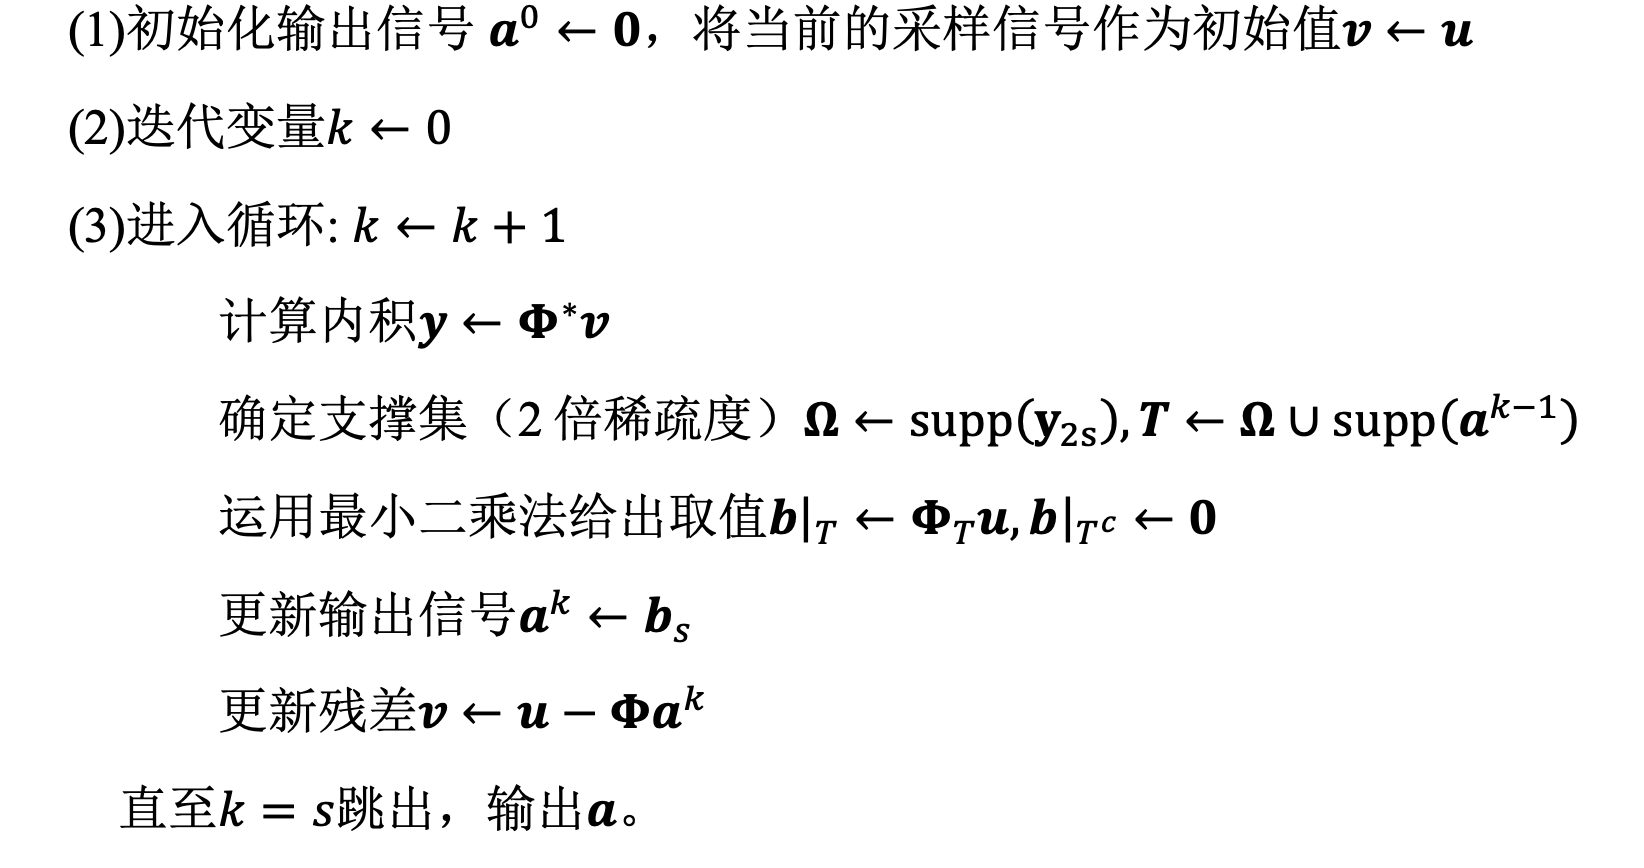
\includegraphics[width=0.8\textwidth]{41.png}
\end{figure}
\section{仿真分析}
这一节我们给出用OMP和CoSaMP两种稀疏重构算法对混沌信号的稀疏采样后还原的仿真结果和分析,其中混沌信号选择为模型
Duffing-WS小世界网络第一个节点的输出,并叠加高斯白噪声。下图给出了 
OMP和CoSaMP两种算法的重构误差关于噪声强度的变化图。可以看到,CoSaMP算法在噪声强度小于0.2时具有非常低的重构误差,
即较好的抗噪重构性能,但之后因噪声强度的增加其误差有快速增长,但其重构性能始终优于经典的OMP算法。
经典的OMP算法对于混沌信号始终存在较大的重构误差。由此可见,CoSaMP算法相较于传统OMP算法有更出色的重构抗噪声能力。
\begin{figure}[!htbp]
    \centering
    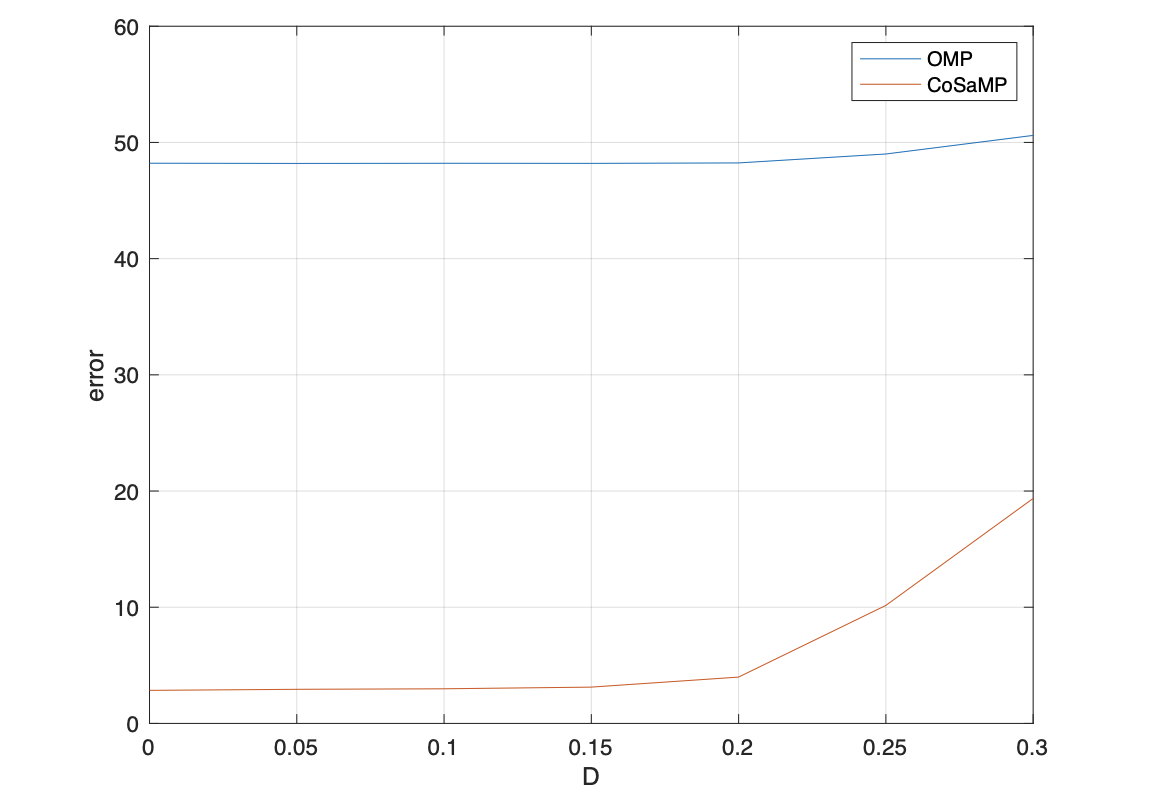
\includegraphics[width=0.6\textwidth]{42.png}
\end{figure}
下图则给出了选择不同稀疏度K值时,OMP和CoSaMP两种算法相应的重构误差。可以看出,CoSaMP算法在稀疏度增加时重构误差显著减小,
在K = 60左右趋于稳定,也说明该混沌信号经过离散傅里叶变换之后的稀疏系数取为60即可较为稳健地恢复该信号,
而OMP算法对该混沌信号的重构能力一直不佳。
\begin{figure}[!htbp]
    \centering
    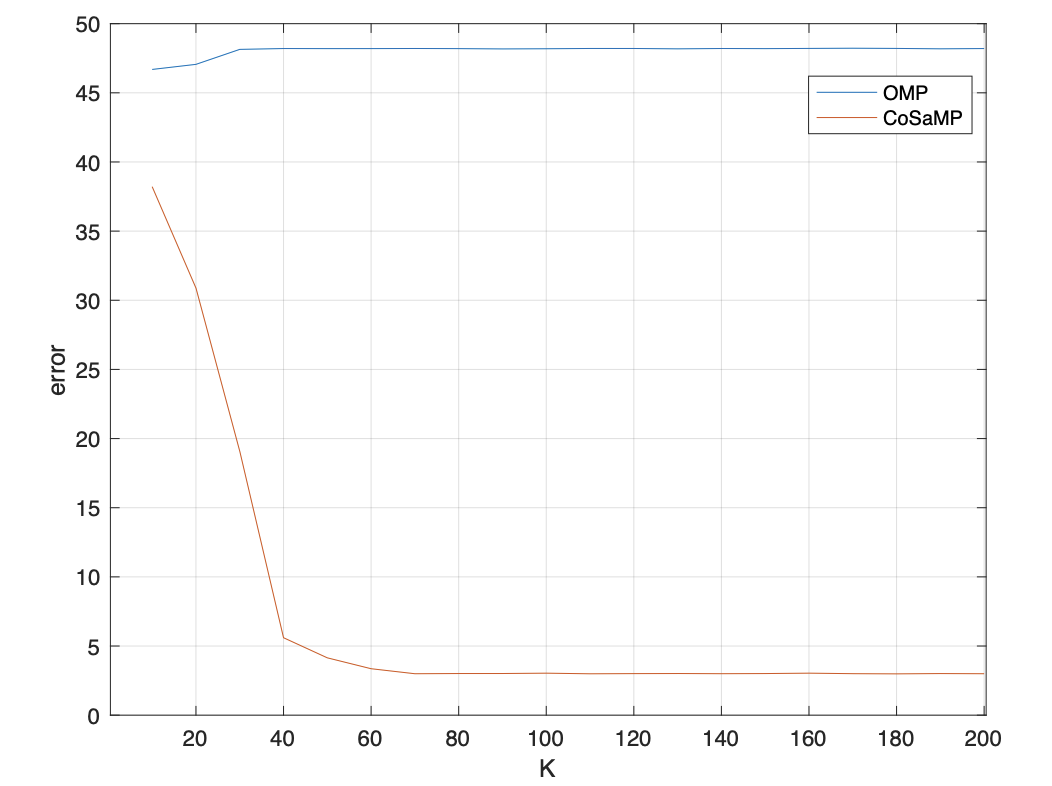
\includegraphics[width=0.7\textwidth]{43.png}
\end{figure}
由此可见,含噪声的混沌信号稀疏重构问题目前尚未有完善的研究,常规的稀疏重构算法也对混沌信号的重构性能不佳,
以OMP算法为例,该算法在常规情况有很好的性能,但是在混沌信号情形的效果不佳。因此对混沌信号重构对传统稀疏重构算法提出了新的挑战。
\section{小结}